\subsubsection{\stid{2.11} LLVM Implementations }

\paragraph{Overview}
The LLVM project is a collection of modular components for building compilers and toolchains.
LLVM comes with support for OpenMP through the C/C++ frontend Clang.
Execution is supported using OpenMP runtime libraries centered around \lstinline{libomp} (for host execution) and \lstinline{libomptarget} (for device execution).
The key focus of this project is to implement OpenMP features in LLVM, enhance features, and provide best-in-class performance with the LLVM community version.
As vendor compilers are built on top of LLVM, enhancements we integrate ``upstream'' are likely to be reused
by one or multiple vendor compilers as well.

We will discuss asynchronous OpenMP offloading in detail now.
Afterwards, we list other recent works and present results of enhanced
OpenMP lowering for GPUs together with OpenMP-aware optimizations.

\paragraph{Key Challenges}

As most of the computational power is within GPUs, it is imperative for performance (per watt) to keep them occupied with productive work at all times. A meaningful approach is to perform as many computations as possible simultaneously. Even Nvidia Fermi GPUs, which have been on the market for ten years, allow for concurrent execution of up to 16 GPU kernels on a single device. Asynchronous offloading is a promising technique to achieve such concurrency as it allows a single CPU thread to overlap memory movement, GPU computation, and the preparation of new GPU tasks on the CPU.
Costly stalls between GPU computations, a.k.a. \emph{kernels}, are avoided and the hardware can start the execution of an already prepared kernel as soon as the ones currently executed stop utilizing the entire device. OpenMP supports asynchronous offloading through the \lstinline|nowait| clause on \lstinline|target| directives, though compiler support still varies.

There are two existing designs that can do asynchronous offloading: regular task and detachable task.
The regular task design is easy to implement, potentially even without compiler support, but it will fail to achieve the goal if there are no threads available to perform the offloading concurrently, which sometimes is unrealistic and restrictive.
The detachable task design can be expected to provide consistently good results under most circumstances.
%However, there are performance challenges with either scheme.
%For one, dependences between host and target tasks need to be handled efficiently.
%While one could resolve host task dependences as part of the setup, thus stalling the encountering thread until they are resolved, it would defeat the purpose.

\paragraph{Solution Strategy}
We propose a new scheme to implement the \lstinline{nowait} clause on \lstinline{target} directives to achieve concurrent offloading.
It is designed to provide good performance regardless of the context.
Our approach utilizes otherwise ``hidden'' helper threads to provide consistent results across various use cases.
In the hidden helper task design, a deferred target task is executed in its entirety by a thread that is not started by nor (in any language-defined way) visible to the user.
These hidden helper threads form a team of threads that is implicitly created at program start and is only responsible for the execution of the special hidden helper tasks.
We denote them in our pseudo code as \lstinline|hht\_task|.
Such tasks are not too different from other deferred OpenMP tasks except that they are always executed by an implicit hidden helper thread.
It is especially important that they participate in the dependence resolution like any other tasks generated by the encountering thread.
Thus they are siblings to tasks generated by threads in the same team as the encountering thread.
The hidden helper task concept is not tied to deferred target task but could help the definition or extension of the OpenMP specification.
\autoref{fig:target_task_intro_split_hht} shows how the generic deferred target task is executed in this design.

\begin{figure}[H]
\begin{lstlisting}[language=C++]
#pragma omp hht_task shared(...) depend(...) ...
#pragma omp target map(...) ...
{ ... }
\end{lstlisting}
\caption{Conceptual lowering of the \lstinline{target} directive to the hidden helper task design.
A special \lstinline{hht_task} is used and executed by an hidden helper thread while the offload part is made synchronous.}
\label{fig:target_task_intro_split_hht}
\end{figure}

Our results show the hidden helper task design gains up to $6.7\times$ improvement on Summit supercomputer, and also provides comparable speedup to the commercial IBM XL C/C++ compiler. Most important, our design provides more functionalities and it can be used even if the native runtime has no asynchronous offloading capabilities.

\begin{figure}[hbt!]
\centering
\subfloat[]{\resizebox{0.45\textwidth}{!}{% This file was created by tikzplotlib v0.9.2.
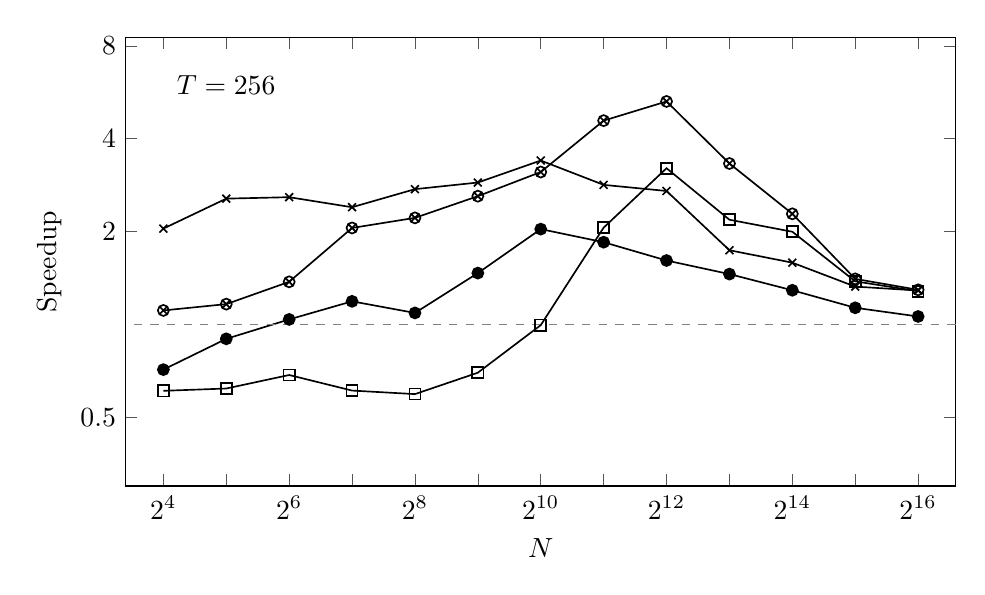
\begin{tikzpicture}

\begin{axis}[
axis line style={black},
xlabel={$N$},
xlabel near ticks,
xmin=-0.6, xmax=12.6,
xtick style={color=white!33.3333333333333!black},
xtick={0,1,2,3,4,5,6,7,8,9,10,11,12},
xticklabels={\(\displaystyle 2^4\),\(\),\(\displaystyle 2^6\),\(\),\(\displaystyle 2^8\),\(\),\(\displaystyle 2^{10}\),\(\),\(\displaystyle 2^{12}\),\(\),\(\displaystyle 2^{14}\),\(\),\(\displaystyle 2^{16}\)},
ylabel={Speedup},
ylabel near ticks,
ytick style={color=white!33.3333333333333!black},
%ytick={0,1,2,3,4,5,6},
%yticklabels={,\(\displaystyle {1.0}\),,\(\displaystyle {3.0}\),,\(\displaystyle {5.0}\),},
%ymin=0.361127455148372, ymax=5.51707532158344,
ymin=0.3, ymax=8.5,
ymode=log,
log basis y={2},
ytick={0.5,2,4,8},
log ticks with fixed point,
width=\textwidth,
height=0.6\textwidth,
title={$T=256$},
title style={below right,at={(0.05,0.9)}}
]
\addplot [semithick, mark=otimes]
table {%
0 1.11147540983607
1 1.16501650165017
2 1.37581699346405
3 2.05629139072848
4 2.21710526315789
5 2.60615384615385
6 3.12078651685393
7 4.57857142857143
8 5.2827140549273
9 3.32571109871723
10 2.28499799438428
11 1.40641665600068
12 1.29619187709406
};
% \addlegendentry{B1}
\addplot [semithick, mark=square]
table {%
0 0.610244988864143
1 0.620842572062084
2 0.686666666666667
3 0.611408199643494
4 0.595488721804511
5 0.698653198653199
6 0.995929443690638
7 2.06111111111111
8 3.21023359288098
9 2.18633540372671
10 1.99912018300194
11 1.38082448735985
12 1.28262231666122
};
% \addlegendentry{B2}
\addplot [semithick, mark=x]
table {%
0 2.04658385093168
1 2.55905511811024
2 2.58680555555556
3 2.4
4 2.74642857142857
5 2.88562091503268
6 3.40054495912806
7 2.83580080753701
8 2.70911949685535
9 1.74132043255549
10 1.58726097495287
11 1.32766260484254
12 1.2893861343636
};
% \addlegendentry{B3}
\addplot [semithick, mark=*]
table {%
0 0.714707329070339
1 0.899248120300752
2 1.03947368421053
3 1.18948412698413
4 1.09095002251238
5 1.46853146853147
6 2.03842794759825
7 1.84909727836163
8 1.61319515399212
9 1.45761636107193
10 1.29182463005992
11 1.13366620453858
12 1.06254475718846
};
% \addlegendentry{B4}
\addplot[gray, dashed] coordinates {(-1,1) (13,1)};
\end{axis}

\end{tikzpicture}
}}
\subfloat[]{\resizebox{0.45\textwidth}{!}{% This file was created by tikzplotlib v0.9.2.
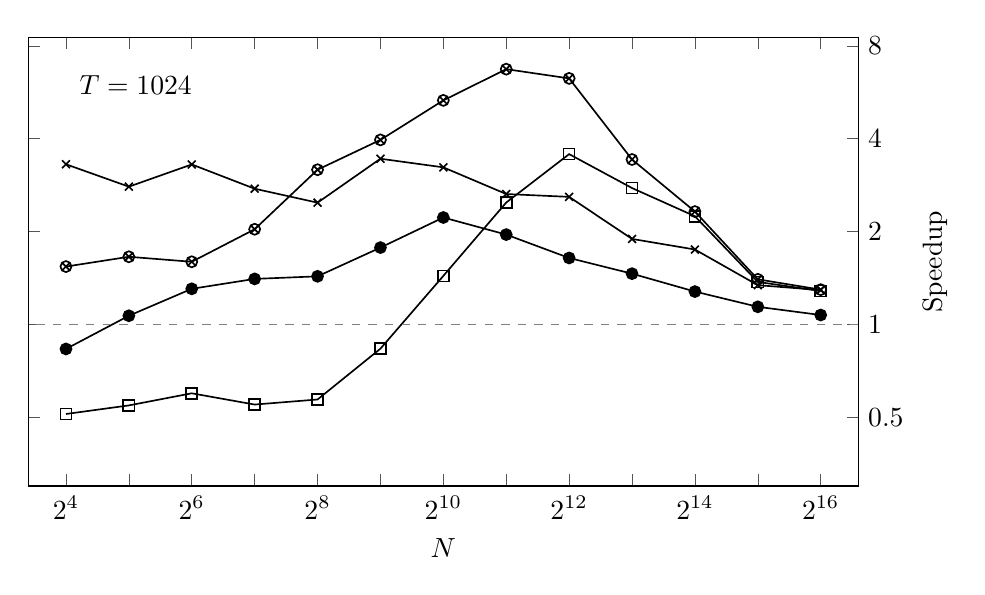
\begin{tikzpicture}

\begin{axis}[
axis line style={black},
xlabel={$N$},
xmin=-0.6, xmax=12.6,
xlabel near ticks,
xtick style={color=white!33.3333333333333!black},
xtick={0,1,2,3,4,5,6,7,8,9,10,11,12},
xticklabels={\(\displaystyle 2^4\),\(\),\(\displaystyle 2^6\),\(\),\(\displaystyle 2^8\),\(\),\(\displaystyle 2^{10}\),\(\),\(\displaystyle 2^{12}\),\(\),\(\displaystyle 2^{14}\),\(\),\(\displaystyle 2^{16}\)},
ylabel={Speedup},
ylabel near ticks,
%ymin=0.202966825333382, ymax=7.6,
ytick style={color=white!33.3333333333333!black},
%yticklabels={,\(\displaystyle {1.0}\),,\(\displaystyle {3.0}\),,\(\displaystyle {5.0}\),,\(\displaystyle {7.0}\),\(\displaystyle {8.0}\)},
ymode=log,
log basis y={2},
ymin=0.3, ymax=8.5,
ytick={0.5,1,2,4,8},
log ticks with fixed point,
yticklabel pos=right,
width=\textwidth,
height=0.6\textwidth,
title={$T=1024$},
title style={below right,at={(0.05,0.9)}}
]
\addplot [semithick, mark=otimes]
table {%
0 1.54172560113154
1 1.65860215053763
2 1.59782608695652
3 2.03624161073826
4 3.17523056653491
5 3.96593673965937
6 5.32525951557093
7 6.72148541114058
8 6.2743450321305
9 3.42638125542378
10 2.32380177063193
11 1.40163487155345
12 1.29789579295094
};
% \addlegendentry{B1}
\addplot [semithick, mark=square]
table {%
0 0.513372472276582
1 0.547333333333333
2 0.599075297225892
3 0.550828729281768
4 0.57201646090535
5 0.835728952772074
6 1.43811764705882
7 2.48555411815438
8 3.56691152986266
9 2.76931747025673
10 2.24389385867926
11 1.37479676536026
12 1.28436651244046
};
% \addlegendentry{B2}
\addplot [semithick, mark=x]
table {%
0 3.30685203574975
1 2.79770114942529
2 3.30263157894737
3 2.75550891920252
4 2.48282630029441
5 3.44634377967711
6 3.23179190751445
7 2.64840182648402
8 2.59288461538462
9 1.89490421158768
10 1.7509535977484
11 1.34198274819622
12 1.29377530790229
};
% \addlegendentry{B3}
\addplot [semithick, mark=*]
table {%
0 0.833864844343204
1 1.06823060410917
2 1.30601343101343
3 1.40609367894497
4 1.4334323922734
5 1.77639399943391
6 2.22291134622401
7 1.9573504027618
8 1.64384220061375
9 1.46215812497777
10 1.27950960037583
11 1.14186188461619
12 1.07420840134936
};
% \addlegendentry{B4}
\addplot[gray, dashed] coordinates {(-1,1) (13,1)};
\end{axis}

\end{tikzpicture}
}}
\caption[]{Speedup of concurrent execution with hidden helper tasks compared to vanilla LLVM with different benchmarks.}
\label{fig:speedup-nw-vanilla}
\end{figure}

\paragraph{Recent Progress}
In recent work we implemented loop transformation constructions introduced in OpenMP 5.1~\cite{kruse2021openmpbooth,kruse2021clangast}, asynchronous offloading for OpenMP~\cite{thiddenhelper}, efficient lowering of idiomatic OpenMP code to GPUs (under review),  OpenMP-aware compiler optimizations with informative and actionable remarks for users (under review), a portable OpenMP device (=gpu) runtime written in OpenMP 5.1 (including atomic support)~\cite{DBLP:conf/iwomp/TianCDC21}, a virtual GPU as debugging friendly
offloading target on the host~\cite{DBLP:conf/icppw/PatelTDC21}, improved diagnostics and execution information~\cite{DBLP:conf/icppw/DoerfertHC21,DBLP:conf/iwomp/HuberWGDH21}.

We redone the OpenMP GPU code generation in LLVM/Clang~\cite{OpenMPEncoding} to improve performance and correctness.
This work was complemented by a new LLVM/OpenMP GPU device runtime that helps us further close the performance gap compared to CUDA and other kernel languages~\cite{NewOpenMPRT}.
Various efforts in improving development and debugging have also been integrated into LLVM/OpenMP~\cite{DBLP:conf/icppw/DoerfertHC21,DBLP:conf/icppw/PatelTDC21}.

We implemented hidden helper task design in LLVM/OpenMP.
Most of our work \cite{DBLP:conf/iwomp/TianCDC21} (except device side dependence resolution) have been upstream and already part of LLVM since 12.0.
Recently Intel also adopted our design and implementation in Intel's latest OpenMP compiler \cite{TianUpdateOnIntelCompiler2021}.

\begin{figure}[tb]
\centering
\subfloat[][Unrolling on AMD EPIC 7532 CPU] ]{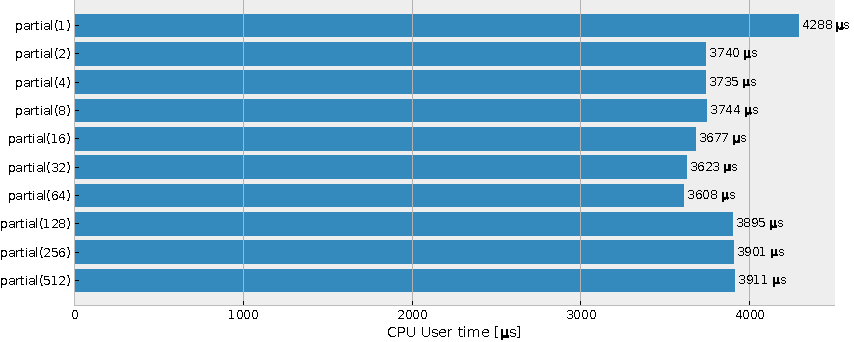
\includegraphics[width=0.5\textwidth]{projects/2.3.2-Tools/2.3.2.11-SOLLVE/unroll.pdf}}%
\subfloat[][Tiling on Intel i5-9400F CPU compared to chunking]{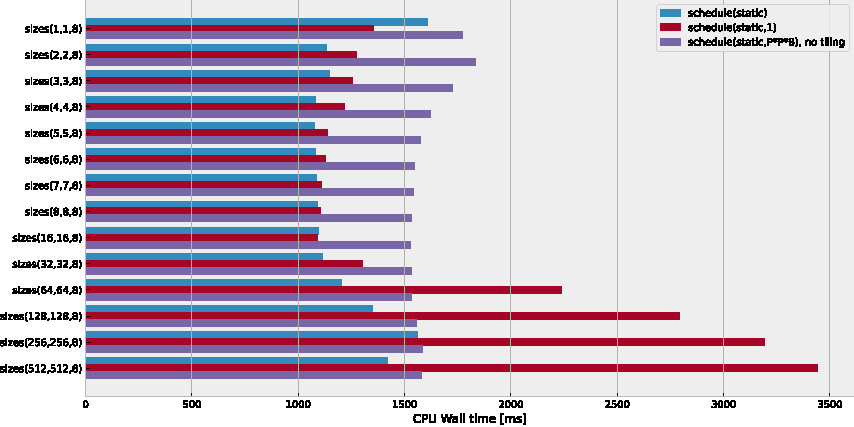
\includegraphics[width=0.5\textwidth]{projects/2.3.2-Tools/2.3.2.11-SOLLVE/tiling.pdf}}
\caption{Performance-Impact of loop transformations on CPUs}
\label{fig:unrolltile}
\end{figure}

The loop transformation constructs implemented in Clang include the \emph{unroll} and \emph{tile} directives.
We demonstrate how these make speedup in the vicinity of 3x (tiling on GPU) and an additional 20\% become
low-hanging fruits by just adding a directive~\cite{kruse2021openmpbooth} as illustrated in \autoref{fig:unrolltile}.
There are actually two implementations, one AST-based and a second using the OpenMPIRBuilder that can also be used other compilers such as Flang~\cite{kruse2021clangast}.

Testing of OpenMP offloading for NVIDIA and AMD GPUs has been added to LLVM's Continuous Integration infrastructure.
This will allow identifying changes that break OpenMP early during development, including those by non-OpenMP developers making maintenance easier.

GPU kernel times have been improved significantly since LLVM 12. \autoref{fig:kernel_times} illustrates the impact of
different optimizations we integrated into LLVM and which are run by default for OpenMP codes. As shown, speedups
of up to 13.35x (RSBench, upper right) were reached while we get closer to CUDA
performance across the board. More recent improvements caused benchmarks like
XSBench (upper left) to also achieve CUDA performance when compiled with OpenMP
offload via our development branch of LLVM/Clang.

\begin{figure}[hbt!]
\centering
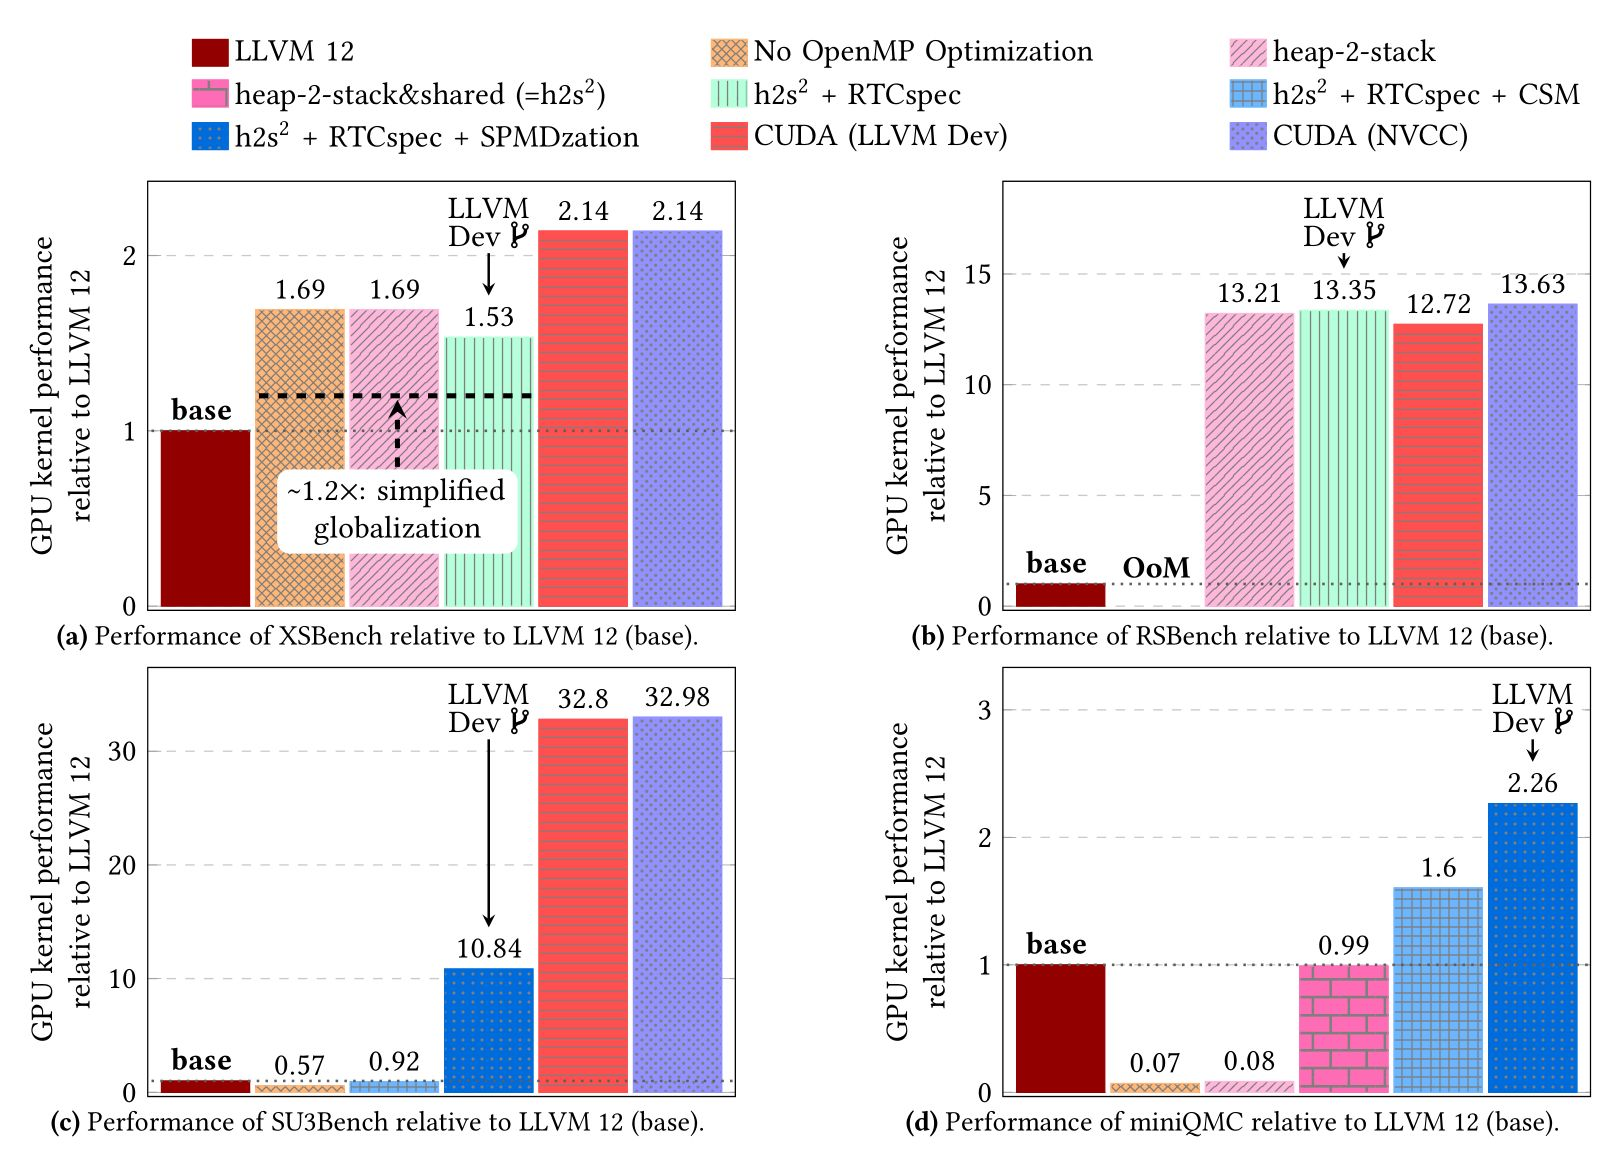
\includegraphics[width=0.95\linewidth]{LLVM-opt-kernel-times.jpg}
\caption[]{Kernel times for different ECP proxy apps when compiled with OpenMP offloading and CUDA. For the former differently optimized versions are shown and the results of a close to LLVM upstream branch is marked explicitly. All times are normalized against LLVM 12 OpenMP offloading performance.}
\label{fig:kernel_times}
\end{figure}

LLVM/Clang 13.0.0 has been officially released on October 4 2021 which includes most of the aforementioned improvements. The branch for LLVM/Clang 14.0.0 has been branched-off the development repository and is expected to be released March 15 2022.


\paragraph{Case study: LLVM/OpenMP performance for OpenMC}

We intensified our work with the OpenMC team on their portable OpenMP implementation of a Monte Carlo code.
Most recent results obtained with LLVM/OpenMP show how our compile enhancements and application engagement improve performance manifold.
Further, the early results on AMD GPUs are very promising and indicate that performance portability is achievable with LLVM/OpenMP.
The performance evolution through our collaboration is summarized in \autoref{fig:openmc}. JLSE testbeds from Argonne National Lab have been used for these results.  
A more detailed report was recently accepted to the PHYSOR conference.


  \definecolor{col0o}{RGB}{0,146,146}
  \colorlet{col0}{col0o!80}
  \definecolor{col1o}{RGB}{182,109,255}
  \colorlet{col1}{col1o!70}
  \definecolor{col2}{RGB}{219,209,0}
  \definecolor{col3}{RGB}{255,182,119}
  \definecolor{col8}{RGB}{182,255,219}
  \definecolor{col5}{RGB}{36,255,36}
  \definecolor{col6}{RGB}{182,219,255}
  \definecolor{col7}{RGB}{255,109,182}
  \definecolor{col18}{RGB}{255,255,109}
  \definecolor{col9}{RGB}{73,0,146}
  \definecolor{col10}{RGB}{146,73,0}
  \definecolor{col11}{RGB}{146,0,0}
  \definecolor{col12}{RGB}{0,109,219}
  \definecolor{col13}{RGB}{0,73,73}
  \definecolor{col14}{RGB}{73,0,73}
  \definecolor{col15}{RGB}{73,73,0}
  \definecolor{col16o}{RGB}{255,36,36}
  \colorlet{col16}{col16o!80}
  \definecolor{col17o}{RGB}{36,36,255}
  \colorlet{col17}{col17o!50}
  \definecolor{col4}{RGB}{255,182,219}
  
  \definecolor{Maroon}{HTML}{990000} 

\begin{figure}[h!]
  \vspace*{3mm}
  \centering

\resizebox{\linewidth}{!}{%
  %\includegraphics{includes/openmc.pdf}

\begin{tikzpicture}
\begin{axis}[
    compat=newest,
    enlarge y limits={rel=0.20},
    enlarge x limits={abs=0.5},
    ybar,
    ymode = log,
    log basis y = 10,
    bar width=40,
    xtick={1,2,3,4,5},
    xticklabels={CPU\\32 cores, A100 initial\\ performance, A100 after application-\\compiler co-design\\ (OpenMC + LLVM), A100 after further\\ algorithmic changes\\ (OpenMC team), AMD MI100 perf-\\ormance latest\\ OpenMC + LLVM},
    xtick style={draw=none},
    xticklabel style={align=center,font=\small},
    %xmajorticks=false,
    ymajorgrids=true,
    ylabel={particles/sec},
    %ylabel style = {align=center,at={(-0.08,0.5)}},
    %yminorgrids=true,
    grid style=dashed,
    height=7cm,
    width=18cm,
    visualization depends on ={y \as \y},
    visualization depends on ={rawy \as \rawy},
    %log ticks with fixed point,
    every node near coord/.append style = {
      %name=a\coordindex,
      %font=\small,
      /pgf/number format/fixed,
      %fill=white,
      %yshift=-2pt,
      %inner sep=0pt,
    },
    every axis plot/.append style={
      bar shift=0pt,
    },
  ]
\addplot[
    %nodes near coords,
    %point meta=rawy,
    nodes near coords={%
      \begingroup%
        % this group is merely to switch to FPU locally.
        % Might be unnecessary, but who knows.
        \pgfkeys{/pgf/fpu}%
        \pgfmathparse{\pgfplotspointmeta<4}%
        \global\let\issmall=\pgfmathresult%
        \pgfmathparse{\pgfplotspointmeta==0}%
        \global\let\iszero=\pgfmathresult%
        \pgfmathparse{\pgfplotspointmeta==1}%
        \global\let\isone=\pgfmathresult%
      \endgroup%
      \pgfmathfloatcreate{0}{0.0}{0}%
      \let\ZERO=\pgfmathresult%
      \pgfmathfloatcreate{1}{1.0}{0}%
      \let\ONE=\pgfmathresult%
      \color{black}%
      \ifx\iszero\ONE%
      {%
        \hspace*{-5mm}%
        \global\let\ycoord=\ZERO%
        \textbf{OoM}%
      }%
      \else%
        \ifx\isone\ONE%
        {%
          \textbf{base}
          \global\let\ycoord=\ZERO%
        }%
        \else%
          \ifx\issmall\ONE%
          {%
            %\global\let\ycoord=\ZERO
            \textbf{\phantom{,}\pgfmathprintnumber[precision=2]{\rawy}\phantom{,}}%
          }%
          \else%
            %\hspace*{-12mm}
            %\hspace*{-4mm}
            %\global\let\ycoord=\rawy
            %\colorbox{white}{%
              \textbf{\pgfmathprintnumber[precision=2]{\rawy}}%
            %}
          \fi%
        \fi%
      \fi%
    },
    every node near coord/.append style = {
        name=a\coordindex,
        /pgf/number format/fixed,
        yshift=0.5pt,
        fill=white,
        inner sep=0pt,
    },
    fill=Maroon,
  ]
  coordinates {
(2,602)
(3,58529)
(4,349685)
};

\addplot[
    %nodes near coords,
    %point meta=rawy,
    nodes near coords={%
      \begingroup%
        % this group is merely to switch to FPU locally.
        % Might be unnecessary, but who knows.
        \pgfkeys{/pgf/fpu}%
        \pgfmathparse{\pgfplotspointmeta<4}%
        \global\let\issmall=\pgfmathresult%
        \pgfmathparse{\pgfplotspointmeta==0}%
        \global\let\iszero=\pgfmathresult%
        \pgfmathparse{\pgfplotspointmeta==1}%
        \global\let\isone=\pgfmathresult%
      \endgroup%
      \pgfmathfloatcreate{0}{0.0}{0}%
      \let\ZERO=\pgfmathresult%
      \pgfmathfloatcreate{1}{1.0}{0}%
      \let\ONE=\pgfmathresult%
      \color{black}%
      \ifx\iszero\ONE%
      {%
        \hspace*{-5mm}%
        \global\let\ycoord=\ZERO%
        \textbf{OoM}%
      }%
      \else%
        \ifx\isone\ONE%
        {%
          \textbf{base}
          \global\let\ycoord=\ZERO%
        }%
        \else%
          \ifx\issmall\ONE%
          {%
            %\global\let\ycoord=\ZERO
            \textbf{\phantom{,}\pgfmathprintnumber[precision=2]{\rawy}\phantom{,}}%
          }%
          \else%
            %\hspace*{-12mm}
            %\hspace*{-4mm}
            %\global\let\ycoord=\rawy
            %\colorbox{white}{%
              \textbf{\pgfmathprintnumber[precision=2]{\rawy}}%
            %}
          \fi%
        \fi%
      \fi%
    },
    every node near coord/.append style={
        /pgf/number format/fixed,
        yshift=0.5pt,
        fill=white,
        inner sep=0pt,
    },
    fill=col6,
  ]
  coordinates {
(1,54913)
};
\addplot[
    %nodes near coords,
    %point meta=rawy,
    nodes near coords={%
      \begingroup%
        % this group is merely to switch to FPU locally.
        % Might be unnecessary, but who knows.
        \pgfkeys{/pgf/fpu}%
        \pgfmathparse{\pgfplotspointmeta<4}%
        \global\let\issmall=\pgfmathresult%
        \pgfmathparse{\pgfplotspointmeta==0}%
        \global\let\iszero=\pgfmathresult%
        \pgfmathparse{\pgfplotspointmeta==1}%
        \global\let\isone=\pgfmathresult%
      \endgroup%
      \pgfmathfloatcreate{0}{0.0}{0}%
      \let\ZERO=\pgfmathresult%
      \pgfmathfloatcreate{1}{1.0}{0}%
      \let\ONE=\pgfmathresult%
      \color{black}%
      \ifx\iszero\ONE%
      {%
        \hspace*{-5mm}%
        \global\let\ycoord=\ZERO%
        \textbf{OoM}%
      }%
      \else%
        \ifx\isone\ONE%
        {%
          \textbf{base}
          \global\let\ycoord=\ZERO%
        }%
        \else%
          \ifx\issmall\ONE%
          {%
            %\global\let\ycoord=\ZERO
            \textbf{\phantom{,}\pgfmathprintnumber[precision=2]{\rawy}\phantom{,}}%
          }%
          \else%
            %\hspace*{-12mm}
            %\hspace*{-4mm}
            %\global\let\ycoord=\rawy
            %\colorbox{white}{%
              \textbf{\pgfmathprintnumber[precision=2]{\rawy}}%
            %}
          \fi%
        \fi%
      \fi%
    },
    every node near coord/.append style={
        /pgf/number format/fixed,
        yshift=0.5pt,
        fill=white,
        inner sep=0pt,
    },
    fill=col3,
  ]
  coordinates {
  (5,93918)
};
\end{axis}

\draw[ultra thick,->,shorten <=1mm,shorten >=3mm] ($(a0.south east) + (3mm,0mm)$) -- node[midway,above,rotate=55,fill=white,inner sep=1pt,yshift=2pt] {97x} ($(a1.south west) + (-0.5mm,1mm)$);
\draw[ultra thick,->,shorten <=1mm,shorten >=3mm] ($(a1.south east) + (3mm,0mm)$) -- node[midway,above,rotate=30,fill=white,inner sep=1pt,yshift=2pt] {6x} (a2.south west);

\end{tikzpicture}
}

\vspace*{-2mm}

\caption{
  Performance results for the OpenMC~\cite{romano2013openmc} OpenMP offloading code that simulates transport of neutral particles using the Monte Carlo methodology.
  The application is part of the ExaSMR ECP project and known for its proxy applications (XSBench~\cite{XS_Tramm_2014} and RSBench~\cite{RS_Tramm_2014}).
  Results show the almost 100x speedup achieved by co-optimizing the full OpenMC application with the LLVM compiler for OpenMP offloading on NVIDIA A100 GPUs.
  In the process, changes to both OpenMC and LLVM were made, and the latter were often triggered via command line options or assumptions.
  Guided by compiler remarks, other applications could benefit similarly and with far less involvement from a compiler developer---but only if the remarks, and later the suggested code changes, are clear, actionable, and effective.
 For context, we also present the AMD MI100 numbers obtained with the latest versions
 of OpenMC and the LLVM/Clang compiler.
 Since the LLVM/OpenMP offloading backend for AMD GPU is new and only recently became stable, we expect substantial performance improvements as we start our tuning efforts.
 Even without, we believe the results shows how performance portability is certainly
 within reach for a full application using the LLVM/OpenMP offloading environment. \\
  The data for the figure was generated and generously provided by John Tramm.
}

  \label{fig:openmc}
  %\vspace*{-2mm}
  \vspace*{2mm}
\end{figure}


\paragraph{Next Steps}
We will keep working on supporting more new OpenMP 5.1 features in LLVM.
%OpenMP 5.1 introduces a number of new features, one of which is new set of useful atomic operations, \lstinline{compare} clause and a combined one \lstinline{compare capture}.
%Now most of atomic operations in scientific applications can be written in OpenMP directly instead of using target dependent intrinsics or function calls.
%We will support the two clauses in LLVM/Clang.
%
To avoid redundant development of two OpenMP implementations, we will mature the development of the OpenMPIRBuilder and make it the default OpenMP code generation for Clang as it is already for Flang.

Improvements to the OpenMP offloading ecosystem are planned, e.g., to extend the remote offloading capabilities we introduced and to further improve development and debugging of OpenMP GPU applications.

More OpenMP-aware optimizations are expected to materialize as we get the last OpenMP benchmarks on par with CUDA performance. We also plan to invest time in generic GPU optimizations soon.

We will implement proof-of-concept implementations of loop transformations that are planned for OpenMP 6.0, such as loop interchange, reversal, fusion, fission and index set splitting.


\paragraph{Experiences on Early Access Systems}

%The SOLLVE team has implemented and optimized an OpenMP offload version of AutoDock-GPU based on a OpenMP CPU OpenMP tasking version, 

AutoDock-GPU is an application code for molecular docking often used to solve problems in the domains of biology and AI/ML on supercomputers including DoE's supercomputers, and it has recently (in 2020 and 2021) been used as the driver for simulations run on supercomputers for developing COVID-19 therapeutics~\cite{legrand2020gpu}. AutoDock-GPU uses OpenMP offload features to run on a single GPU and has the ability for parallelize and schedule computation across multiple GPUs on a node through OpenMP. The OpenMP offload implementation of AutoDock-GPU was developed by members of the SOLLVE team. The application code has been experimented with using LLVM 12 OpenMP and LLVM 13 OpenMP on one node of the Spock Early Access System provided by ECP. Note that the LLVM 13 results were not in our SOLLVE FY21 Program Review slides and we only showed LLVM 12 then.

Figure~\ref{fig:llvmadspck} shows the wall clock timings of AutoDock-GPU when using 3 different sizes of ligands on one GPU of Spock, under LLVM OpenMP 12 and LLVM OpenMP 13. The results show that LLVM 13 OpenMP (rocm4.5) improves performance over LLVM 12 OpenMP (rocm4.2) of the AutoDock-GPU for the largest problem size, i.e., the 3er5 ligand, by 16.56\%. The results show that the LLVM OpenMP implementation version generally has an impact to performance and suggests has a larger impact with larger problem size for this application. 

\begin{figure}[h!]
    \centering
    \subfloat[One GPU. \label{fig:llvmadspck}] {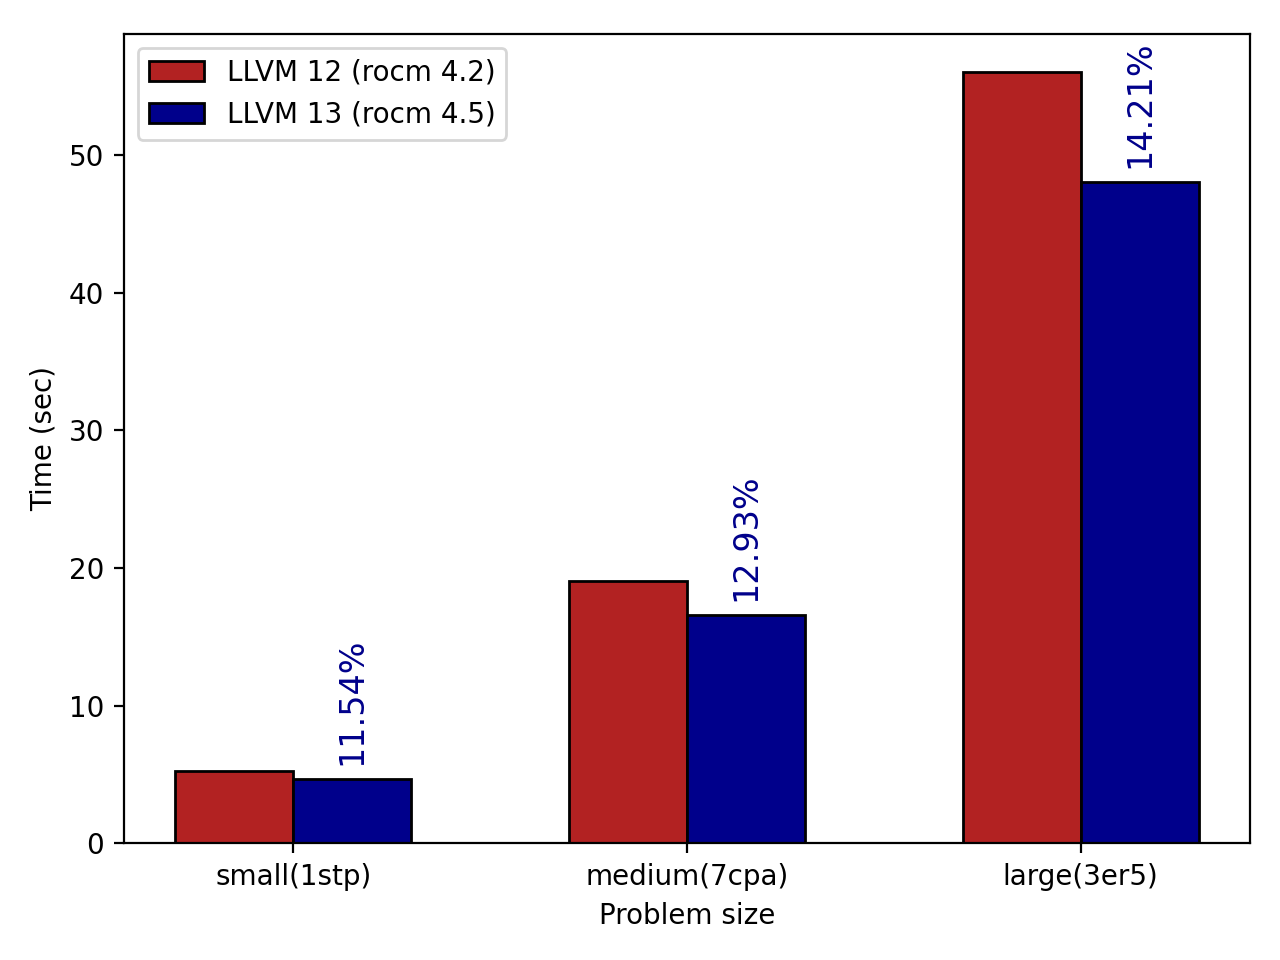
\includegraphics[scale=0.5]{projects/2.3.2-Tools/2.3.2.11-SOLLVE/one_gpu_spock.png}}\subfloat[One node (four GPUs). \label{fig:mgpuSpock} ]{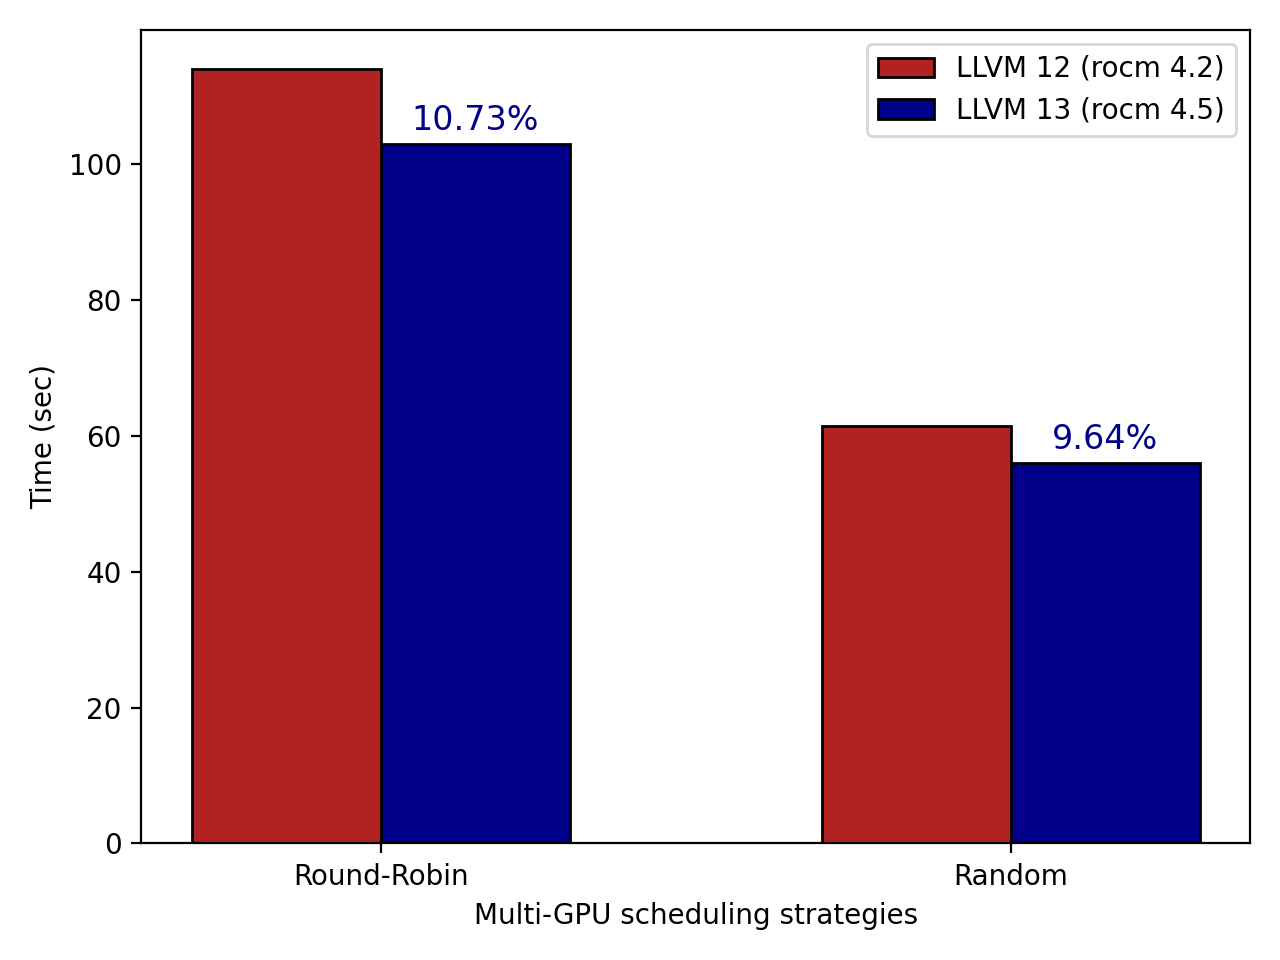
\includegraphics[scale=0.5]{projects/2.3.2-Tools/2.3.2.11-SOLLVE/multi_gpu_spock.png}}
    \caption{Running AutoDock-GPU with LLVM's OpenMP on Spock.} 
\end{figure}

Figure~\ref{fig:mgpuSpock} shows results for strategies for an OpenMP parallelization of AutoDock-GPU (using an assortment of the three ligands in Figure~\ref{fig:llvmadspck}) across the 4 GPUs of Spock. The figure specifically shows the difference in performance between a static assignment of the application's computation to GPUs and a dynamic assignment - or scheduling - of the application's computation across multiple GPUs of the node, as discussed in~\cite{9669317}, and the impact of the LLVM OpenMP implementation version. The round-robin scheduler under LLVM 13 OpenMP (rocm4.5) improves performance over the round-robin scheduler in LLVM 12 OpenMP (rocm4.2) by 10.73\%. Under LLVM 13’s OpenMP (rocm4.5), using a dynamic assignment (labeled \textit{random} in Figure~\ref{fig:mgpuSpock} and where OpenMP chunks of a loop are assigned to randomly chosen GPU) as opposed to a static assignment (labeled \textit{round-robin} in Figure~\ref{fig:mgpuSpock} and where OpenMP chunks are assigned to a GPU based on chunk number) cuts the execution time by 45.63\%. By using the newer LLVM 13 over LLVM 12 and by using the \textit{random} multi-GPU scheduling strategy instead of the \textit{round-robin} scheduling strategy, AutoDock-GPU is sped up by approximately 2.05x. Using the dynamic multi-GPU scheduling strategy over the static one improves performance 4.5 times more than using the new LLVM OpenMP implementation version over the older one, but the newer LLVM OpenMP implementation version still helps improve performance substantially and by about 10\%. 